\section{Cyclomatic complexity}

\begin{definition}[Graph homology]
    Let $G = (V,E)$ be a directed graph. The corresponding integral simplicial chain complex is $C(G; \mathbb Z) = (C_*, \partial_*)$ where
    \[ C_0 = \mathbb Z \langle V \rangle, \qquad C_1 = \mathbb Z \langle E \rangle \]
    and $C_i = 0$ for all $i \geq 2$ and the only non-trivial boundary map $\partial: C_1 \to C_0$ is defined by
    \[ \partial(v, w) = w - v, \]
    and extending linearly. The \emph{$n$th homology group of $G$} is simply the $n$th homology group of $C(G; \mathbb Z)$; that is,
    \[
        H_n(G) = H_n(C(G)) =
        \begin{cases}
            \coker\partial & n = 0,            \\
            \ker\partial   & n = 1,            \\
            0              & \text{otherwise}.
        \end{cases}
    \]
\end{definition}

\begin{proposition} \label{prop:graph-homology}
    Let $G = (V,E)$ be a graph and $C$ be the set of connected components of $G$. Then the graph homology of $G$ is given by
    \[
        H_n(G) = \begin{cases}
            \mathbb Z^{\lvert C \rvert}                                     & n  = 0,           \\
            \mathbb Z^{\lvert E \rvert + \lvert C \rvert - \lvert V \rvert} & n = 1,            \\
            0                                                               & \text{otherwise}.
        \end{cases}
    \]
    That is, the rank of the first homology is the number of connected components in $G$ and the rank of the second homology is the number of linearly independent cycles in $G$ (the concept of linearly independent paths is later formalised).
\end{proposition}

\begin{proof}
    Recall that $H_0(G) = \ker \partial_0 / \im \partial_1$. Now we consider a component of $G$. We see that any vertex can be obtained by another vertex by adding elements of $\im \partial_1$. Thus all vertices belong to the same equivalence class. It is clear that we cannot do the same for two vertices within different components, thus $H_0(G) \cong \Z^{\lvert C \rvert}$. Now we let $T \subset E'$ be a spanning tree of a component $G' = (V', E')$. We observe that if we add another edge (not in $T$) to $T$, we get a cycle. Thus each edge in $E' \setminus T$ corresponds to a cycle in $G'$. $\lvert E' \setminus T \rvert = \lvert E' \rvert - (\lvert V' \rvert - 1)$. Considering every component, we get $H_1(G) \cong \Z^{\lvert E \rvert - \lvert V \rvert + \lvert C \rvert}$. The rest of the homology groups is trivial, given that the boundary map is trivial.
\end{proof}

\begin{definition}[Control-flow graph]
    A \emph{control-flow graph} of a program is a directed graph $G = (V,E)$ where
    \begin{enumerate}
        \item each vertex $v \in V$ corresponds to a block (piece of code) without any jumps; and
        \item each edge $(v,w) \in E$ corresponds to a jump in the control flow (that is, the order in which statements are executed).
    \end{enumerate}
    We designate two special types vertices:
    \begin{enumerate}
        \item $v_{\text{en}}$: the \emph{entry block}, in which control enters the graph; and
        \item $v_{\text{ex}}$: the \emph{exit block}, in which control leaves the graph.
    \end{enumerate}
\end{definition}

\begin{figure}
    \makebox[\textwidth][c]{
        \begin{subfigure}{0.37\textwidth}
            \centering
            \includegraphics{content/5-applications/images/control-flow-ex-1}
            \caption{The control flow graph of an if-else.}
            \label{fig:control-flow-ex-1}
        \end{subfigure}
        \hspace{0.01\textwidth}
        \begin{subfigure}{0.37\textwidth}
            \centering
            \includegraphics{content/5-applications/images/control-flow-ex-2}
            \caption{The control flow graph of a while loop.}
            \label{fig:control-flow-ex-2}
        \end{subfigure}
        \hspace{0.01\textwidth}
        \begin{subfigure}{0.37\textwidth}
            \centering
            \includegraphics{content/5-applications/images/control-flow-ex-3}
            \caption{The control flow graph of an if-elseif-else.}
            \label{fig:control-flow-ex-3}
        \end{subfigure}
    }
    \caption{Control-flow graphs of some simple programs.}
    \label{fig:control-flow-ex}
\end{figure}

Here, we will only be considering graphs in which there exists a path from the entry block to every other block. Figure \ref{fig:control-flow-ex} shows examples of control-flow graphs for some simple programs.

\begin{definition}[Linearly independent paths]
    Let $G = (V,E)$ be a directed graph and $Q$ a set of paths in $G$. $Q$ is said to be \emph{linearly independent} if, for each $p \in Q$, there is an edge in $p$ that is not included in any other path $q \in Q \setminus \{p\}$. $Q$ is said to be a \emph{basis} of $G$ if it is maximal.
\end{definition}

It is simple exercise to prove that all bases of a graph $G$ have the same cardinality.

\begin{example}
    Consider the graph drawn below.
    \begin{center}
        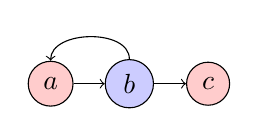
\begin{tikzpicture}[main/.style = {draw, circle}]
            \node[main, fill=red!20] (1) {$a$};
            \node[main, fill=blue!20] (2) [right of=1] {$b$};
            \node[main, fill=red!20] (3) [right of=2] {$c$};
            \draw[->] (1) to (2);
            \draw[->] (2) to [out=90, in=90] (1);
            \draw[->] (2) to (3);
        \end{tikzpicture}
    \end{center}
    One example of a set of linearly independent paths (from $a$ to $c$) is
    \[ Q = \{(a,b,c), (a,b,a,b,c)\} \]
    and indeed this set forms a basis. But the set
    \[ Q' = \{(a,b,a,b,c), (a,b,a,b,a,b,c)\}\]
    is not linearly independent as every edge in the second path is present in the first path.
\end{example}

\begin{definition}[Cyclomatic complexity]
    Consider a program $P$ and let $G$ be its control-flow graph. The \emph{cyclomatic complexity} of $P$, denoted $M(P)$, is the number of linearly independent paths from the entry block to the exit block in $G$.
\end{definition}

\begin{example}
    \hspace{0em}
    \begin{enumerate}
        \item For the control-flow graphs shown in Figure \ref{fig:control-flow-ex-1} and Figure \ref{fig:control-flow-ex-2}, $M(P) = 2$.
        \item For the control-flow graph shown in Figure \ref{fig:control-flow-ex-3}, $M(P) = 3$.
    \end{enumerate}
\end{example}

\begin{lemma} \label{lem:bijection-paths-cycles}
    Let $P$ be a program, $G$ its control-flow graph, $Q$ be a basis of paths between $v_{\text{en}}$ and $v_{\text{ex}}$ in $G$, and $C$ be a basis of cycles based at $v_{\text{en}}$ in $G/{\{v_{\text{en}}, v_{\text{ex}}\}}$. Then
    \[ \lvert Q \rvert = \lvert C \rvert. \]
\end{lemma}

\begin{proof}
    Let $p = (v_{\text{en}}, v_1, \ldots, v_n, v_{\text{ex}}) \in Q$. Then the induced path (from $G$ to $G/{\{v_{\text{en}}, v_{\text{ex}}\}}$) $\overline p$ is clearly a cycle, and we claim that it is linearly independent. Assume otherwise, then for all $\overline e \in \overline p$ there is a path $\overline p_{\overline e} \in \overline Q$ such that $\overline e \in \overline p_{\overline e}$. As $G$ is simple, the quotient map forms a bijection between the edges of $G$ and the edges of $G/{\{v_{\text{en}}, v_{\text{ex}}\}}$ (and thus a bijection between the paths). Thus for all $e \in p$, there is a path $p_e \in Q$ such that $e \in p_e$ and therefore, $Q$ is not linearly independent; a contradiction. We also claim that $\overline Q$ is maximal. Indeed, let $\overline c$ be a cycle in $G/{\{v_{\text{en}}, v_{\text{ex}}\}}$ such that $\overline Q \cup \{\overline c\}$ is linearly independent. But then $Q \cup \{c\}$ is linearly independent, and so $Q$ is not maximal; a contradiction.
\end{proof}

Figure \ref{fig:control-flow-identified-ex} shows the control flow graph $G$ of an if-elseif-else program, alongside the quotient graph $G/\{v_{\text{en}}, v_{\text{ex}}\}$.

\begin{figure}
    \makebox[\textwidth][c]{
        \begin{subfigure}{0.37\textwidth}
            \centering
            \includegraphics{content/5-applications/images/control-flow-ex-3}
            \caption{The control flow graph $G$ of an if-elseif-else program.}
            \label{fig:control-flow-ex-3-2}
        \end{subfigure}
        \hspace{0.01\textwidth}
        \begin{subfigure}{0.37\textwidth}
            \centering
            \includegraphics{content/5-applications/images/control-flow-identified}
            \caption{The quotient graph $G/{\{v_{\text{en}}, v_{\text{ex}}\}}$.}
            \label{fig:control-flow-identified}
        \end{subfigure}
    }
    \caption{Control-flow graphs of some simple programs.}
    \label{fig:control-flow-identified-ex}
\end{figure}

The following is a direct result from Proposition \ref{prop:graph-homology} and Lemma \ref{lem:bijection-paths-cycles}.

\begin{corollary}
    Let $P$ be a program and $G = (V,E)$ be its control-flow graph. Then
    \[ M(P) = \rank H_1(G, \{v_{\text{en}}, v_{\text{ex}}\}) = \lvert E \rvert + 2\lvert C \rvert - \lvert V \rvert \]
    where $C$ is the connected components of $G$.
\end{corollary}

Cyclomatic complexity is a commonly used metric for the testability of code, and our persistent homology algorithm presents an efficient method for its computation. 
